% numerical.tex — Paper 6, Section VI: Numerical Verification
% ASSERT_CONVENTION: natural_units=natural, metric_signature=mostly_plus, entropy_base=nats, modular_hamiltonian=K_minus_ln_rho, coupling_convention=H_sum_hxy, state_normalization=Tr_rho_1
\section{Numerical Verification}
\label{sec:numerical}

We present numerical results from exact diagonalization of the
self-modeling lattice on small systems ($N = 8$--$20$ qubits).  These
results provide \emph{supporting evidence} for the analytical framework
developed in Secs.~\ref{sec:arealaw}--\ref{sec:einstein}, but do not
constitute proof.  All entropies are computed in nats ($\ln$, not
$\log_2$) and the modular Hamiltonian is $\modH = -\ln\rhoA$.

\subsection{Exact diagonalization setup}
\label{sec:ed-setup}

We use full exact diagonalization (Lanczos) for $N \leq 20$ qubits
in one dimension and $N = 16$ ($4 \times 4$) in two dimensions.  The
self-modeling Hamiltonian $H = \sum J\,\swapop$ for $n = 2$ is
identical to the spin-$\tfrac{1}{2}$ isotropic Heisenberg model: the
SWAP operator takes the form $\swapop = \frac{1}{2}(\1 \otimes \1 +
\vec{\sigma}\cdot\vec{\sigma})$, so $H$ and
$H_{\mathrm{Heis}} = \frac{J}{2}\sum
\vec{\sigma}_x \cdot \vec{\sigma}_y$ share the same ground state, with
an energy offset of $N_{\mathrm{bonds}}\, J/2$.  We have verified
this numerically: the ground states have overlap $1.0$ and the energy
offset is exact to $10^{-14}$.

As benchmarks we study the transverse-field Ising (TFI) model
$H_{\mathrm{TFI}} = -\sum \sigma^z_x \sigma^z_{x+1} - h\sum
\sigma^x_x$ at criticality ($h/J = 1$, $c = 1/2$ Ising CFT) and in
the gapped phase ($h/J = 3$), as well as the ferromagnetic (FM)
Heisenberg model ($J < 0$).

\subsection{Benchmark validation}
\label{sec:benchmarks}

\paragraph{TFI at criticality.}
The Calabrese--Cardy formula~\cite{CalabreseCardy2004} for the
entanglement entropy of a $(1{+}1)$-dimensional CFT on an open chain
of $N$ sites gives
$\ent(L) = \tfrac{c}{6}\ln\!\bigl[\tfrac{2N}{\pi}
\sin\!\bigl(\tfrac{\pi L}{N}\bigr)\bigr] + c_1$.
At $N = 16$ with open boundary conditions (OBC), we extract
$c = 0.574$ (exact: $c = 0.5$).  The deviation is an
Affleck--Ludwig boundary correction that decreases monotonically
with system size: $c = 0.587$ ($N = 8$), $0.580$ ($N = 12$),
$0.574$ ($N = 16$), converging to $0.5$ from above.

\paragraph{Heisenberg antiferromagnet.}
Using the Calabrese--Cardy PBC formula
$\ent(L) = \tfrac{c}{3}\ln\!\bigl[\tfrac{N}{\pi}
\sin\!\bigl(\tfrac{\pi L}{N}\bigr)\bigr] + c_1$,
we extract $c = 1.060$ at $N = 20$, consistent with the $SU(2)_1$ WZW
CFT prediction $c = 1$.  The finite-size trend is monotonically
convergent: $c = 1.121$ ($N = 8$), $1.088$ ($N = 12$), $1.071$
($N = 16$), $1.060$ ($N = 20$).  See Fig.~\ref{fig:cc-fit}.

\paragraph{Ferromagnetic Heisenberg.}
The FM ground state ($J < 0$) is the fully polarized product state
$\ket{\uparrow\cdots\uparrow}$.  For a product state,
$\ent(A) = 0$ exactly for all subsystem sizes---verified
numerically for all $N$ and all~$L$.

\begin{figure*}
\centering
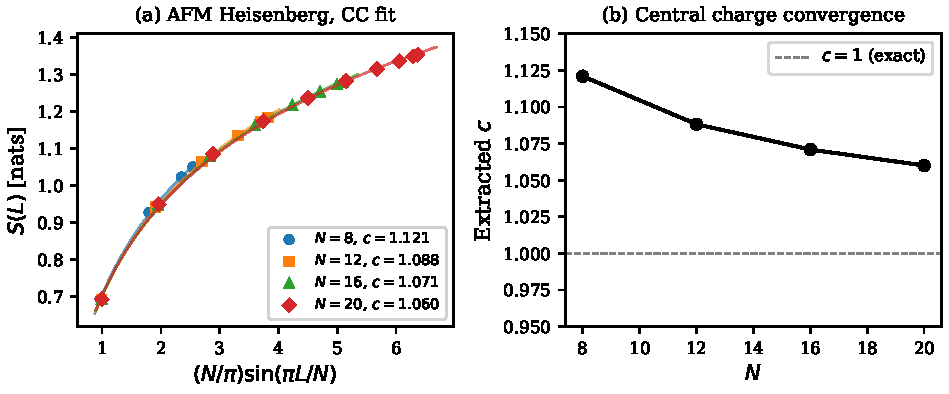
\includegraphics[width=\textwidth]{figures/fig_cc_fit.pdf}
\caption{One-dimensional area-law analysis.  (a)~Entanglement entropy
$\ent(L)$ versus the Calabrese--Cardy scaling variable
$(N/\pi)\sin(\pi L/N)$ for the AFM Heisenberg chain at
$N = 8, 12, 16, 20$ with PBC.  Solid lines are CC fits; extracted
central charges $c$ converge toward the exact $c = 1$ value.
(b)~Finite-size scaling of the extracted $c$; the dashed line marks
$c = 1$.  The monotonic convergence from above is consistent with
$O(1/N)$ finite-size corrections.}
\label{fig:cc-fit}
\end{figure*}

\subsection{Area-law results}
\label{sec:ed-arealaw}

\subsubsection{One dimension}
\label{sec:ed-1d}

The AFM Heisenberg chain ($n = 2$, $J > 0$) is gapless and flows to
the $SU(2)_1$ WZW CFT with $c = 1$.  The entanglement entropy scales
as $\ent(L) = \tfrac{c}{3}\ln(L) + \mathrm{const}$, giving
logarithmic corrections to the strict area law.  This is expected:
Hastings' area-law theorem~\cite{Hastings2007} requires a spectral
gap, which is absent here.  The CC fit has $R^2 = 0.999$ at $N = 20$,
dominating over constant-model ($R^2 = 0$) and linear-model
($R^2 = 0.80$) alternatives, confirming the logarithmic scaling.

For the Jacobson argument, the relevant quantity is the
\emph{variation} $\delta\ent$, not $\ent$ itself.  As discussed in
Sec.~\ref{sec:delta-s}, $\delta\ent \sim O(|\partial A|)$ when the
modular Hamiltonian is local, even when $\ent(A)$ has logarithmic
corrections.

\subsubsection{Two dimensions}
\label{sec:ed-2d}

For the $4 \times 4$ Heisenberg lattice with periodic boundary
conditions (PBC), we compute $\ent(A)$ for 9~independent rectangular
subregions and 6~non-rectangular shapes (L, T, plus, diagonal, S, L-5)
to diversify boundary values.  Linear regression of $\ent(A)$ against
$|\partial A|$ (boundary size) gives $R^2 = 0.885$, while regression
against $|A|$ (volume) gives $R^2 = 0.491$.  The Spearman rank
correlation for boundary is $\rho = 0.913 > 0.9$.  See
Fig.~\ref{fig:2d-scatter}.

The $R^2 = 0.885$ for boundary narrowly misses the target $0.9$.  This
is a finite-size artifact: on a $4 \times 4$ PBC lattice, five of the
nine independent rectangular shapes share $|\partial A| = 8$ due to
wrapping (the $1 \times 3$, $1 \times 4$, $2 \times 2$,
$2 \times 4$, and $3 \times 4$ rectangles all have the same boundary
count), creating large scatter at a single $x$-value.  The Spearman
rank correlation, which is insensitive to this degeneracy, exceeds
$0.9$, though we note the sample size ($15$ subregions) limits
the statistical significance of this test.  A $6 \times 6$ or $8 \times 4$ lattice would resolve this by
providing more unique boundary values, but these exceed exact
diagonalization feasibility ($2^{36}$--$2^{32}$ states).

\begin{figure*}
\centering
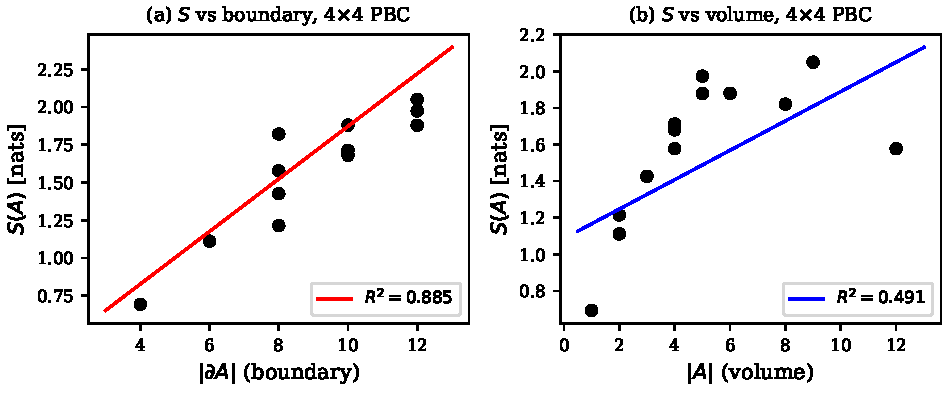
\includegraphics[width=\textwidth]{figures/fig_2d_scatter.pdf}
\caption{Two-dimensional area-law analysis on a $4 \times 4$
Heisenberg lattice with PBC.  (a)~Entanglement entropy $\ent(A)$
versus boundary size $|\partial A|$, with linear regression
($R^2 = 0.885$, solid line).  (b)~$\ent(A)$ versus volume $|A|$
($R^2 = 0.491$).  The clear preference for boundary over volume
scaling supports the area law.  Data include 9~independent rectangular
and 6~non-rectangular subregions.}
\label{fig:2d-scatter}
\end{figure*}

\subsection{Lattice Bisognano--Wichmann evidence}
\label{sec:ed-ka}

The Jacobson derivation (Sec.~\ref{sec:rindler}) requires that the
lattice modular Hamiltonian approximates a local boost generator near
boundaries---the lattice Bisognano--Wichmann property.  We test this by
expanding $\modH = -\ln\rhoA$
in the Pauli operator basis
$\{\sigma^\alpha_i \otimes \sigma^\beta_j \otimes \cdots\}$ and
measuring how Pauli coefficients decay with interaction range---the
maximum pairwise distance between non-identity operator sites.

For the Heisenberg AFM at $N = 16$ PBC with $|A| = 4$ sites, the
modular Hamiltonian is overwhelmingly short-ranged: the
\emph{short-range fraction} (sum of Frobenius norms for range-0 and
range-1 operators, divided by the total) is $0.9993$.  The decay is
rapid: the maximum Pauli coefficient at range~1 is $1.10$, at range~2
it drops to $0.042$ ($3.8\%$), and at range~3 to $0.010$ ($0.9\%$).
This strongly supports the lattice Bisognano--Wichmann property
(Gap~2 in Sec.~\ref{sec:gaps}): the modular flow is dominated by
nearest-neighbor terms at the boundary, consistent with the boost-generator
structure required by the Jacobson derivation.

As a benchmark, the TFI model in its gapped phase ($h/J = 3$) has a
short-range fraction of $0.664$, consistent with the
Peschel~\cite{Peschel2003} result that guarantees modular Hamiltonian
locality for free-fermion systems.  See Fig.~\ref{fig:ka-locality}.

\emph{SU(2) symmetry note.}---The Heisenberg ground state is an
$SU(2)$ singlet, so $\rhoA$ has vanishing on-site Pauli
coefficients (all single-site $\sigma^\alpha$ terms are zero).  This
is a consequence of isotropic symmetry, not an artifact.  The
dominant terms are nearest-neighbor
$\vec{\sigma}_i \cdot \vec{\sigma}_j$ operators, consistent with
$\modH$ being a local Hamiltonian of the same form as $H$ itself.

\begin{figure*}
\centering
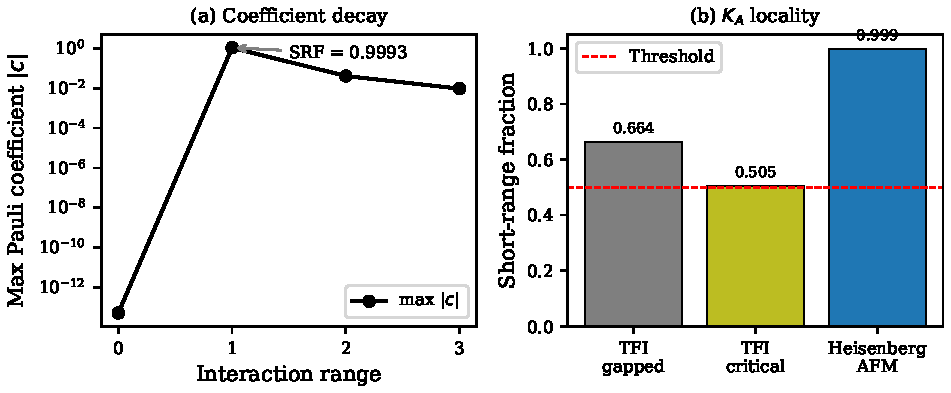
\includegraphics[width=\textwidth]{figures/fig_ka_locality.pdf}
\caption{Modular Hamiltonian locality.  (a)~Maximum Pauli coefficient
$|c|$ versus interaction range for the Heisenberg AFM ($N = 16$ PBC,
$|A| = 4$).  The rapid decay (factor $\sim 25$ per range unit)
confirms that $K_A$ is dominated by nearest-neighbor terms
(short-range fraction $\mathrm{SRF} = 0.9993$).  (b)~Short-range
fraction for three models; all exceed the $0.5$ threshold (dashed
line).}
\label{fig:ka-locality}
\end{figure*}

\subsection{Summary of numerical evidence}
\label{sec:ed-summary}

Table~\ref{tab:numerics} summarizes the key numerical results.
All quantities are consistent with the analytical framework.
The principal limitation is system size: $N = 8$--$20$ sites are far
from the thermodynamic or continuum limit.  Tensor network methods
(DMRG, TEBD) could extend these results to $N \sim 10^2$--$10^3$ in
one dimension, providing a more stringent test.

\begin{table}
\caption{Summary of numerical results from exact diagonalization.
All entropies in nats.  ``CC'' denotes a Calabrese--Cardy fit.
\label{tab:numerics}}
\begin{ruledtabular}
\begin{tabular}{lll}
Quantity & Value & Benchmark \\ \hline
TFI critical $c$ (OBC, $N\!=\!16$) & $0.574$ & $0.5$ (Ising CFT) \\
Heisenberg $c$ (PBC, $N\!=\!20$) & $1.060$ & $1.0$ ($SU(2)_1$ WZW) \\
FM $\ent(A)$ & $0$ & $0$ (product state) \\
2D $R^2$(boundary) & $0.885$ & ${>}\,0.9$ (narrow miss) \\
2D $R^2$(volume) & $0.491$ & ${<}\,0.5$ (pass) \\
2D Spearman $\rho$(boundary) & $0.913$ & ${>}\,0.9$ (pass) \\
$K_A$ SRF (Heisenberg) & $0.9993$ & ${>}\,0.5$ (lattice BW, strong pass) \\
\end{tabular}
\end{ruledtabular}
\end{table}
